\newpage
\section{Approfondimenti tecnologici}\label{ApprofondimentiTecnologici}
	
	\subsection{Webhook}
    I webhook sono un pattern HTTP leggero che fornisce un modello publisher/subscriber semplice
    per collegare tra loro Web API.	
    Quando si verifica un evento in un servizio, viene inviata una
    notifica ai sottoscritti registrati sotto forma di una richiesta HTTP. La richiesta contiene informazioni sull'evento che rende possibile per il ricevitore agire di conseguenza.
    Le tecnologie Redmine e GitLab li integrano e utilizzando una specifica porta, dove i nostri
    Producer sono in ascolto, viene inviato un file \gloss{Json} contenente tutte le informazioni riguardanti l'evento.
    Questa tecnologia ha forma tale da fornirci collezioni di dati organizzati, facilitandoci così la lettura e la scrittura.\par
    % Per quanto riguarda i file JSON usiamo un \gloss{dizionario python} chiamato obj, contiene i campi interessanti e sono:
    Seguono \gloss{dizionari Python} chiamati genericamente \texttt{obj} contenenti i campi dei webhook di nostro interesse:
    \begin{itemize}

            \item GitLab Issue Event:
        \begin{lstlisting}[language = json]
   obj["object_kind"]
   obj["project"]["id"]/obj["object_attributes"]["project_id"]
   obj["project"]["name"]
   obj["assignees"][k]["nome utente"]
   obj["object_attributes"]["action"]
   obj["object_attributes"]["description"]
   obj["labels"][k]["title"]
   obj["labels"][k]["project_id"]
   obj["changes"]["title"]
   obj["changes"]["labels"]["previous"][k]["title"]
   obj["changes"]["labels"]["current"][k]["title"]
        \end{lstlisting}

            \item GitLab Push Event:
        \begin{lstlisting}[language = json]
    obj["object_kind"]
    obj["utente_id"]
    obj["utente_nome utente"]
    obj["project_id"]
    obj["commits"][k]["id"]
    obj["commits"][k]["message"]
    obj["commits"][k]["timestamp"]
    obj["commits"][k]["author"]["name"]
    obj["total_commits_count"]
        \end{lstlisting}

            \item Redmine Issue Event:
        \begin{lstlisting}[language = json]
    obj["payload"]["issue"]["priority"]["name"]
    obj["payload"]["issue"]["tracker"]["name"]
    obj["payload"]["issue"]["subject"]
    obj["payload"]["issue"]["status"]["name"]
    obj["payload"]["issue"]["description"]
    obj["payload"]["issue"]["project"]["id"]
    obj["payload"]["issue"]["project"]["name"]
    obj["payload"]["issue"]["action"]
        \end{lstlisting}
    \end{itemize}

		\subsection{Redmine}
		Ciascuna istanza di Redmine permette l'utilizzo di webhook%
        \footnote{Riferirsi alla voce ``Webhook di Redmine'' alla sezione \S\ref{sec:RiferimentiInformativi}}
        che inviano segnalazioni al Producer alla modifica del progetto.
        Queste vengono ricevute dal server tramite una componente che resta in ascolto,
        aggiornando in base a ciò che riceve dai dati presenti sul Gestore Personale e inoltrando i messaggi
        ai Consumer interessati.
		
		\subsection{GitLab}
		Ciascuna istanza di GitLab, online o in un server locale,
        mette a disposizione la configurazione di webhook\footnote{Riferirsi alla voce ``Webhook di GitLab'' alla sezione \S\ref{sec:RiferimentiInformativi}}
        che, alla modifica di una repository, manda un messaggio con le informazioni relative a quell'evento specifico.
        Questo messaggio arriva a una componente applicativa capace di
        aggiornare i dati presenti nel Gestore Personale e, come per Redmine, inoltrare le notifiche ai Consumer interessati.
		
		\subsection{Apache Kafka}
		Apache Kafka è un software \gloss{open source} che permette la lettura e la scrittura di messaggi su differenti canali di comunicazioni per i dati.
		Questi messaggi arrivano dai Producer che ricevono le notifiche di applicazioni di terze parti immettendole nel Broker. Questo le elabora analizzandone
        il contenuto e contrassegnandole con Topic che verranno utilizzati per l'inoltro ai Consumer e successivamente agli utenti finali, i quali possono abbonarsi a più Topic.
		
		\subsection{Telegram}
		Telegram permette l'interazione in maniera automatica con gli utenti tramite
        bot\footnote{Riferirsi alla voce ``Bot di Telegram'' alla sezione \S\ref{sec:RiferimentiInformativi}}
        che possono essere configurati per mandare messaggi ricevuti da strumenti di terze parti, in questo caso \progetto.
        Il Consumer interroga il Broker per acquisire i messaggi da inoltrare e li trasmette al bot di Telegram, che si
        occuperà dell'invio all'utente finale.

		\subsubsection{BotFather}
		Per mandare messaggi tramite Telegram all'utente finale, è necessario utilizzare un bot creato con BotFather.
        Quest'ultimo è esso stesso un bot offerto da Telegram che permette la creazione e la configurazione di bot che
        possono fare da tramite tra utenti
        e servizi esterni dai quali ricevere, o a cui mandare, informazioni o comandi.

		\subsection{Email}
		Per inoltrare le Email agli utenti finali utilizziamo un Consumer associato che sfrutta il \gloss{server SMTP} di posta
        in modo tale da poter inoltrare i messaggi ottenuti dal Broker all'indirizzo specificato.

		\subsection{Docker}
		L'azienda ci consiglia di utilizzare \gloss{Docker} per la semplicità di utilizzo e per l'adattamento all'architettura a microservizi.
		La configurazione avverrà tramite un \gloss{Dockerfile} in cui verranno specificate informazioni come sistema operativo, script di avvio,
        numero di istanze ed altri parametri specifici.
        
        \subsubsection{Container software}\label{TecnologieContainer}
        
        Un \gloss{container software} simula un ambiente virtuale dove è possibile testare e mantenere le proprie applicazioni, permettendo di aumentare l'efficienza riducendone i costi e simulando l'esecuzione di sistema operativo su una macchina con \gloss{risorse} condivise.
        
        \paragraph{Differenza tra container e macchina virtuale}
        A differenza delle \gloss{macchine virtuali}, dove lo stato dell'ambiente viene salvato su disco, occupando memoria, i container si adattano in maniera più performante all'applicativo richiesto, in quanto il loro scopo è quello di massimizzare la quantità delle applicazioni in esecuzione riducendo al minimo il numero delle macchine per eseguirla.
        Sono quindi più leggeri, occupando meno memoria su disco e impiegando meno risorse.
        
        \subsubsection{DockStation}
        Per la gestione dei container in locale è stato possibile utilizzare \gloss{DockStation} in quanto fornisce una GUI dalla quale si possono effettuare i comandi impartiti a Docker via Terminale.
        \'E inoltre possibile avere la visione dello stato di ciascun container e vedere in tempo reale i log che questo genera, oltre che a poter controllare le risorse utilizzate da ciascun container.
        
        \subsection{Rancher}
    	Per la gestione dei container in remoto, la proponte \II~ci ha messo a disposizione un \gloss{cluster} con due server sui quali è stato installato Rancher. Questo è un software di gestione di oggetti di \gloss{Kubernetes} che fornisce un'interfaccia grafica più ricca rispetto a quella di Dockstation e funzionalità maggiori.
    	Da qui possiamo quindi gestire i nostri container installando le immagini direttamente dal \glossary{DockerHub} senza aver bisogno di file di configurazione come ad esempio quello necessario al docker-compose.
    	
    	\begin{figure}[H]
    		\centering
    		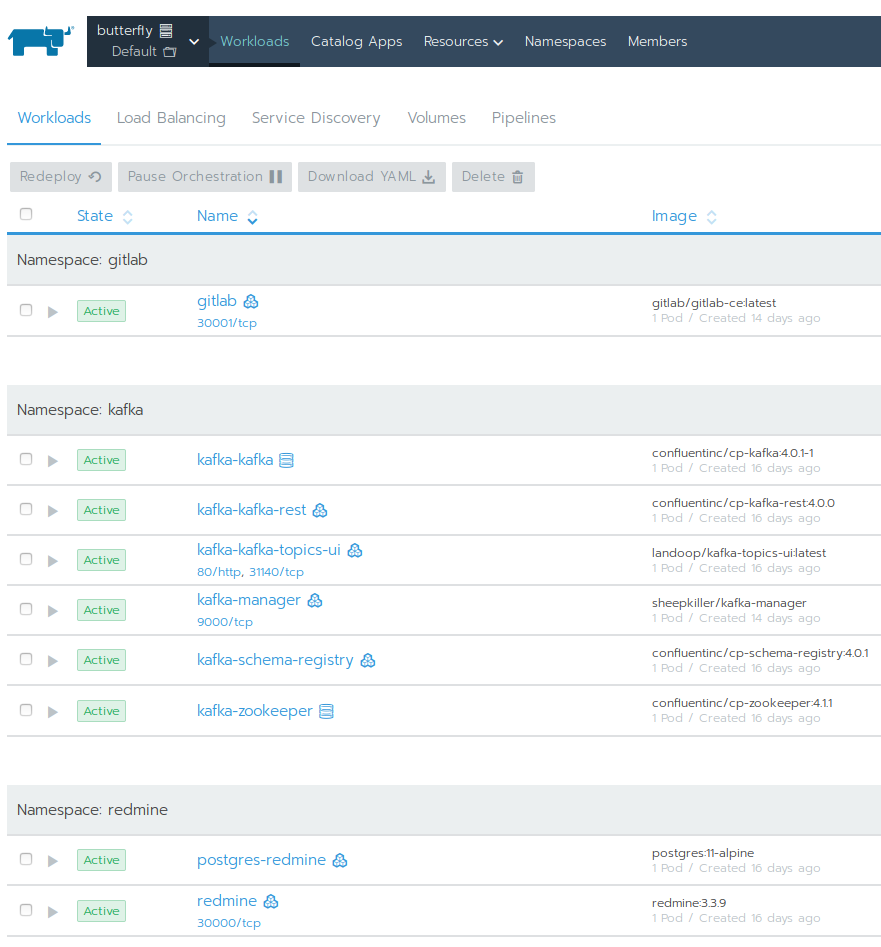
\includegraphics[width=.7\textwidth]{img/rancher.png}\\
    		\caption{Alcuni servizi attivi su Rancher}
    		\label{fig:rancher}
    	\end{figure}
        
			